\section{Conclusion}
The different combinations of M\=/forms and discourse U\=/forms
which are found in Amarasi are summarised in \trf{tab:SumUfoMfoCom}.
Metathesis in Amarasi is a morphological
device used to signal whether a situation, event, or communicative act is resolved or not.
U\=/forms are used to signal a lack of resolution,
with more information being required to achieve such resolution.

\begin{table}[h]
	\caption[Summary of U\=/form and M\=/form combinations]{Summary of U\=/form and M\=/form combinations\su{†}}\label{tab:SumUfoMfoCom}
	\centering
		\begin{threeparttable}[b]
			\stl{0.3em}\begin{tabular}{rccccccc} \lsptoprule
							& decl. clause	& Dep. Coord.	& THL					& Poetry			& Chiasmus	& Q/A					& Conv.	\\ \midrule
					M M	& ✔		&							& 			&\srf{sec:PoePar}	&				& \srf{sec:Q/A}	&						\\
					U M	&		& \srf{sec:DepCoo}			&				&\srf{sec:PoePar}	&						& \srf{sec:Q/A}	& \srf{sec:MaiInt}\\
					U U	&								&							&							&							&						&							&\\
					M U	&								&							&							&							&						&							&(\srf{sec:MaiInt})\\
				M M M &	✔		&							&							&							&						&							& \srf{sec:MaiInt}\\
				U M M &								&							& \srf{sec:UforTaiMforHea}	&							&						&							&						\\
				U U M &								&							& \srf{sec:UforTaiUforHea}	&							&						&							& \srf{sec:MaiInt}\\
				M U M &								&							& \srf{sec:MforTaiUforHea}	&							& \srf{sec:CenChi}&			&						\\
				U M U &								&							&							&							&						&							&						\\
				M M U &								&							&							&							&						&							&						\\
				M U U &								&							&							&							&						&							&						\\
				U U U &								&							&							&							&						&							& (\srf{sec:MaiInt})\\
			\lspbottomrule
			\end{tabular}
			\begin{tablenotes}
				\item [†] decl. clause = declarative clause,
												Dep. Coord. = Dependent Coordination,
												THL = Tail-head linkage,
												Q/A = question-answer pairs,
												Conv. = Conversation
			\end{tablenotes}
		\end{threeparttable}
\end{table}

\trf{tab:SumUfoMfoCom} shows that nearly
all combinations of an M\=/form and a discourse U\=/form
have an M\=/form as the final element.
U\=/forms are canonically resolved by an M\=/form.
This is seen most clearly in tail-head linkage (\srf{sec:TaiHeaLin}),
question-answer pairs (\srf{sec:IntUnm}), and poetic parallelisms (\srf{sec:PoePar}) 
in all of which U\=/forms are obligatorily resolved by M\=/forms.
It is also seen in dependent coordination (\srf{sec:DepCoo}) and chiasmus (\srf{sec:CenChi})
in which U\=/forms are usually resolved by M\=/forms.

A discourse U\=/form entails the presence of a
corresponding M\=/form somewhere in the discourse.
The use of a U\=/form obliges the speaker
or other discourse participants to supply an M\=/form
to complete the discourse structure in which both occur.
At the discourse level, U\=/forms and M\=/forms
comprise a parallel and complementary pair of morphological forms;
they are a dyadic set, with each form being one half of a whole.
The complementary and parallel nature of discourse U\=/forms and M\=/forms
in Amarasi is represented in Figure \ref{fig:AmaDisMet}.

\begin{figure}[h]
	\caption{Amarasi discourse metathesis}\label{fig:AmaDisMet}
	\centering{\Huge
		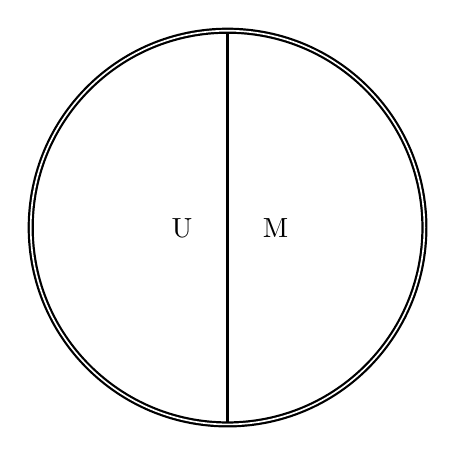
\begin{tikzpicture}[scale=.5]
			\draw[thick,double] (0,0) circle (5);
			%\draw[thick] (-5,0) -- (5,0);
			\draw[thick] (0,-4.95) -- (0,4.95);
				\node[label={[label distance=2mm]180:U}] at (0,0) {};
				\node[label={[label distance=2mm]360:M}] at (0,0) {};
		\end{tikzpicture}}
\end{figure}
